\documentclass[11pt]{article}

\usepackage{graphicx, epsfig}
\usepackage{amsmath, amssymb, latexsym}
\usepackage[english]{babel}
\usepackage{amssymb}   
%\usepackage{graphicx}
%\usepackage{float} 






% Make a larger page (shrink the margins)
%
\setlength{\textwidth}{6.7in}
\setlength{\textheight}{9.0in}
\setlength{\evensidemargin}{0.0in}
\setlength{\oddsidemargin}{0.0in}
\topmargin -0.5in
\footskip 0.5in



\title{Weekly Report for August 3rd}
\author{Eric Davis}
\begin{document}
\maketitle
\medskip



\section{Time Profiles}
\hspace{0.5cm}

I managed to improve the Gillam's missing data for a better Gaussian fit. Unfortunately, the Gaussfit function does not handle -NaN's well, and would not fit a curve with the missing data. However, I made missing data do an average of the data above and below it (in time), and it seems like a completely reasonable and accurate method. I updated all the Gillam time profiles. The comparison you can see in figure 1 and 2.

\begin{figure}[h!]
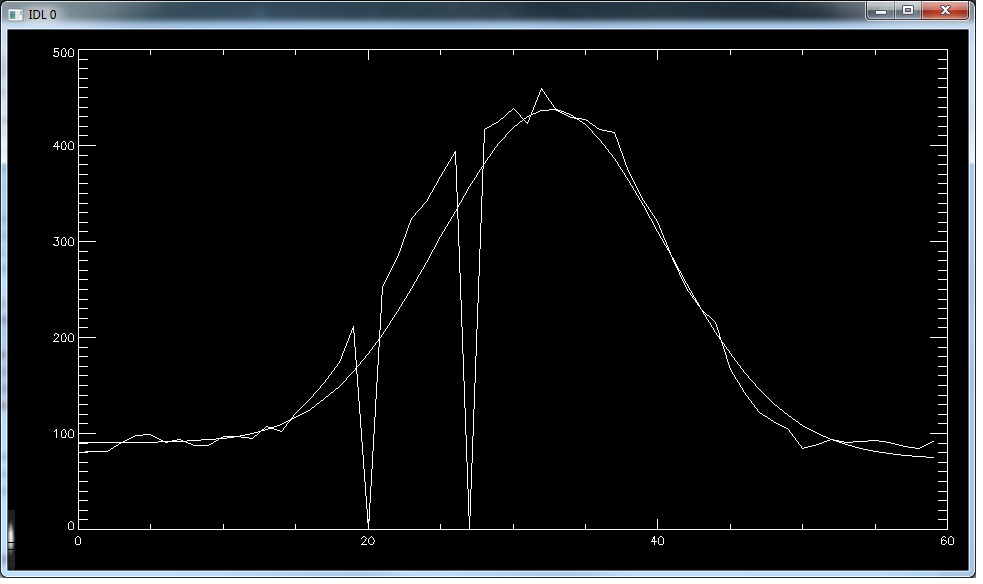
\includegraphics[scale=0.6]{gillam_jupiter_filled_data_11_20_2011.jpg}
\caption{An example of the Gillam data that was filled in with just zeroes. Messes up the Gaussfit enough to justify improving the code}
\end{figure}


\begin{figure}[h!]
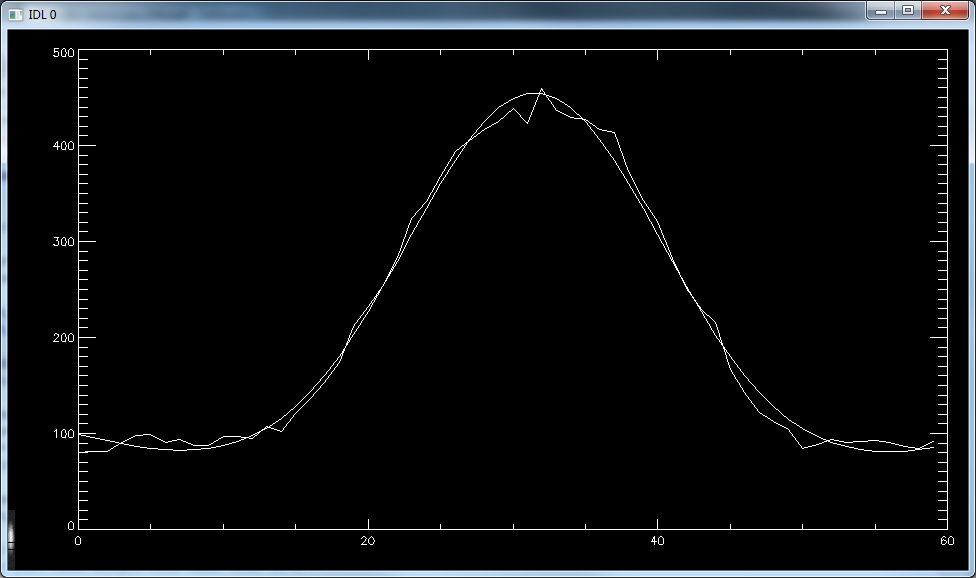
\includegraphics[scale=0.6]{gillam_average_fill.jpg}
\caption{This is the fit with the data averaged. Seems more Gaussian and the program does not try and fit the zeros into the curve for a more accurate result.}
\end{figure}


\section{Comparing the FWHM of the sites}

I compiled all the FWHM data from the four sites, as well as the heights of the profiles above the background, onto one spreadsheet. I then produced plots of FWHM's for all the filters except filter 6 (unreliable results) as a function of site latitude. Choosing site latitude was arbitrary, but it does demonstrate some disturbing results. All FWHM's are averaged over at least 5 nights of data, with outliers being excluded. The thought process being there is always a chance of some random atmospheric affect messing up the profile.  Pinawa consistently has a FWHM that is generally about 1 minute shorter than the other three sites across all seven filters, which are generally consistent with one another. The FWHM is always at least 30 seconds shorter than the other sites. We will need to discuss why this is the case, as currently I am fairly stumped what could be causing this besides an error with the optics of the imager. 

\begin{figure}[h!]
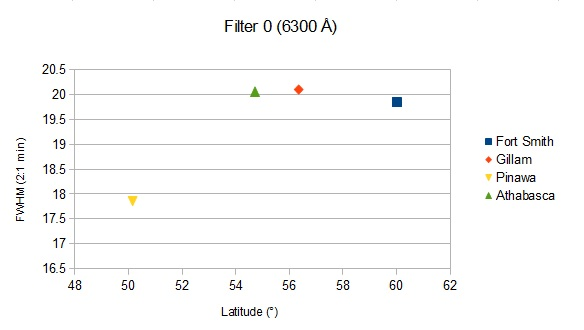
\includegraphics[scale=1.0]{filter0_FWHM.jpg}
\end{figure}

\begin{figure}[h!]
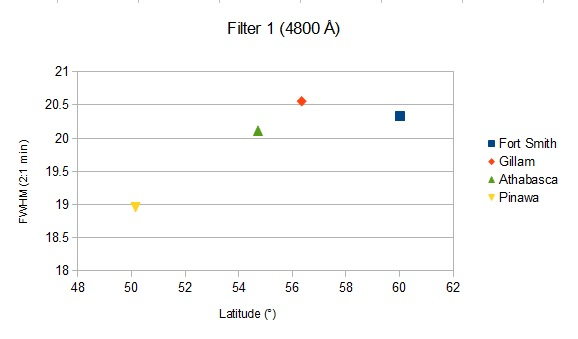
\includegraphics[scale=1.0]{filter1_FWHM.jpg}
\end{figure}

\begin{figure}[h!]
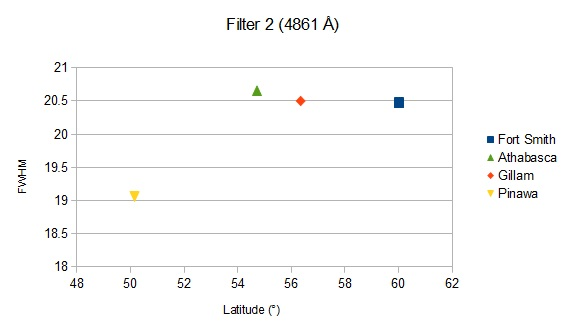
\includegraphics[scale=1.0]{filter2_FWHM.jpg}
\end{figure}

\begin{figure}[h!]
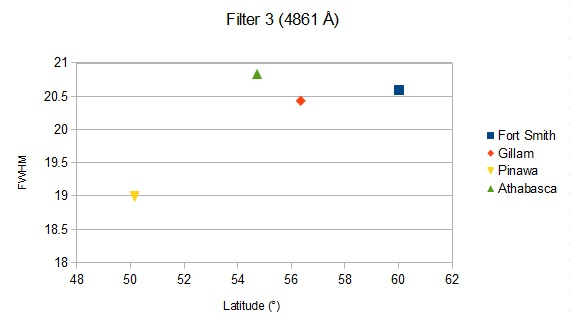
\includegraphics[scale=1.0]{filter3_FWHM.jpg}
\end{figure}

\begin{figure}[h!]
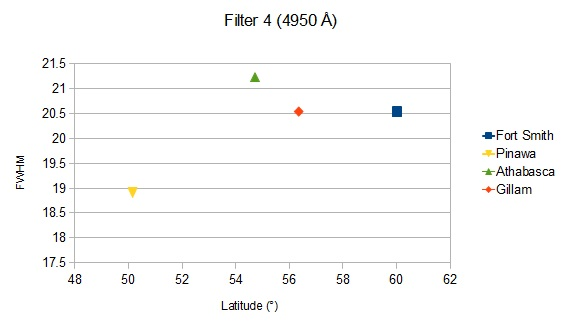
\includegraphics[scale=1.0]{filter4_FWHM.jpg}
\end{figure}

\begin{figure}[h!]
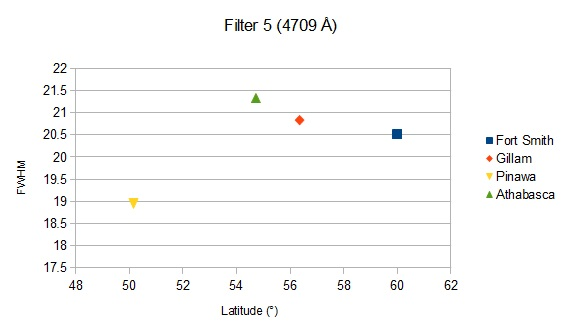
\includegraphics[scale=1.0]{filter5_FWHM.jpg}
\end{figure}

\begin{figure}[h!]
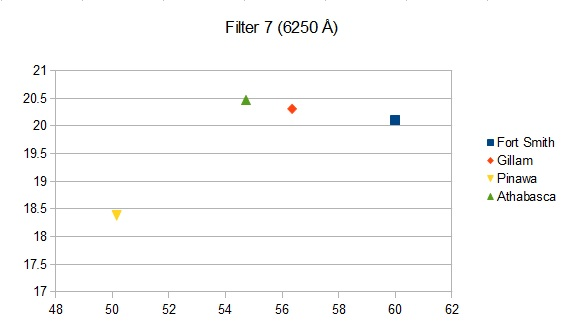
\includegraphics[scale=1.0]{filter7_FWHM.jpg}
\end{figure}


\section{Space Profiles}
\hspace{0.5cm}

I have also started a spreadsheet with space profiles of Jupiter. By having enough space profiles, in theory we should be able to calibrate with very little uncertainty the exact direction the all sky camera is pointed. However, Jupiter tends to occupy a very similar spot in the sky over short periods. I am trying to produce space profiles as far apart from each other as possible, but at this point in time it is somewhat limited by the data. Jupiter is generally only visible at night at the four sights from September to February, and data that's from over a year old often only has data from Gillam or Fort Smith. I am hoping that space profiles over approximately six months is enough to map out where the all sky camera is looking. 



\section{Future Considerations}
\hspace{0.5cm}

Next week I want to continue with the space profiles. As well, I want to try and look for a causal link with why Pinawa's time profiles are not consistent with the rest. I will probably be talking to you about this. By the end of next week I should have enough space profiles of Jupiter to try and figure out exactly where the cameras are pointed. 

\end{document}
\end{article}